\documentclass[11pt,a4paper,ngerman]{report}
\usepackage{babel}
\usepackage{float}
\usepackage[utf8]{inputenc}
\usepackage[T1]{fontenc}
\usepackage{amsmath}
\usepackage{amssymb}
\usepackage{graphicx}
\usepackage{subfig}
\usepackage{csquotes}
\usepackage[backend=bibtex,natbib=true,style=alphabetic]{biblatex}
\addbibresource{Quellen.bib}

\date{\today}
\title{Belegarbeit zur Quellencodierungsmethode \textbf{"Run-Length Encoding"} im Modul "statistische Nachrichtentheorie"}
\author{Von: Monique Golnik (563075) \\ \\Dozent: Prof. Dr. Christoph Lange \\Master Informations- und Kommunikationstechnik WS 2021/22}

\begin{document}

	\maketitle
	\tableofcontents

	\chapter{Einleitung}
	In der heutigen Zeit ist es wichtiger den je sich mit der Komprimierung von Daten auseinander zu setzen. Dateien wie Bilder, Kurzvideos  oder Musik gewinnen zunehmend an Beliebtheit und werden datentechnisch immer größer. Ein schnelles Senden zu jemand anderem gehört dabei mittlerweile zum Alltag.  Auch wenn die gegenwärtige Speicherkapazität einem das Gefühl der Grenzenlosigkeit vermittelt, entspricht dies nicht der Realität - Kompressionsverfahren sind nicht mehr wegzudenken und gewinnen stetig an Bedeutung.  
	
	Gegenstand dieser Belegarbeit ist die nähere Betrachtung des Codierverfahrens \textbf{Run-Length Encoding}.
	Ziel ist es, dass ein Verständnis der Funktionsweise dieser Methode und dessen Grenzen vermittelt werden.
    
	Zunächst wird in Kapitel 2  in die Thematik  eingeführt und die grundlegenden Begrifflichkeiten der QuellenCodierung und Datenkompression definiert. In Kapitel 3 wird das Verfahren \textbf{Run-Length Encoding} erläutert, Vor- und Nachteile abgeschätzt sowie Anwendungsbeispiele dargestellt, um den Einsatz zu verdeutlichen.



	\chapter{Quellencodierung und Datenkompression}
	
		Bei der Quellencodierung ist es das Ziel, dass die Symbolentropie erhöht und so die Redundanz reduziert wird. Sie ist eine eineindeutige Darstellung der Quelleninformation in einer realisierbaren und möglichst redundanzfreien beziehungsweise -armen Form.
		
		Die Aufgabe der Quellencodierung besteht darin einen Datensatz, der von einer Informationsquelle abgegeben wurde, in einen Binärcode mit möglichst kleiner Stellenzahl zu codieren. \cite[Seite 47 ff.]{Lange2021}
	     
	    \enquote{Bei der Datenkompression werden Dateien in eine alternative Darstellung überführt, die effizienter ist als die ursprüngliche. Ziel dieser Codierung ist es, sowohl den benötigten Speicherplatz als auch die Übertragungszeit zu verringern.} \cite{IONOS} 
	
		Durch zwei unterschiedliche Ansätze, lässt sich so ein Codiergewinn erreichen:
	
		\begin{itemize}
		\item \textbf{Redundanz-Kompression}: 
		Auf der Grundlage einer Redundanzreduktion lassen sich Daten nach der Kompression verlustfrei wieder dekomprimieren - eine solche Kompression ist nur möglich, wenn ein Datensatz sich wiederholende Zeichen beinhaltet
		
		\item \textbf{Irrelevanz-Kompression}:
		Bei diesem Ansatz werden irrelevante Informationen entfernt, um einen Datensatz zu komprimieren. Jedoch lässt sich dieser dadurch nicht Bit-genau wiederherstellen und ist somit verlustbehaftet
		\end{itemize}
	
	
		Im Folgenden Kapitel wird der Fokus auf die verlustfreie Kompressionsmethode \textbf{Run-Length Encoding} gerichtet und näher betrachtet.
	
	
	\chapter{Run-Length Encoding}	
  		\section{Redundanz-Kompression durch RLE}
  		
  		
  		  Die Lauflängencodierung \footnote{(Run-Length Encoding (RLE), Run-Length Coding (RLC), Lauflängencodierung = Synonyme} beschreibt eine verlustfreie Kompression, die sinnvoll angewandt werden kann, wenn der gesendete Datensatz Sequenzen mit sich mehrfach wiederholenden Zeichen enthält.
  		  
  		  
  		  Die RLE ist den sogenannten \textbf{Phrasencodern} zugeordnet, wie in Abbildung \ref{MMK} dargestellt. Bei diesen wird nicht wie bei den Entropiecodern auf den mittleren Informationsgehalt geachtet, sondern auf eine syntaktische Einheit, die abgeschlossen ist.
  		  
  		  \begin{figure} [H]
  		  	\begin{center}
  		  		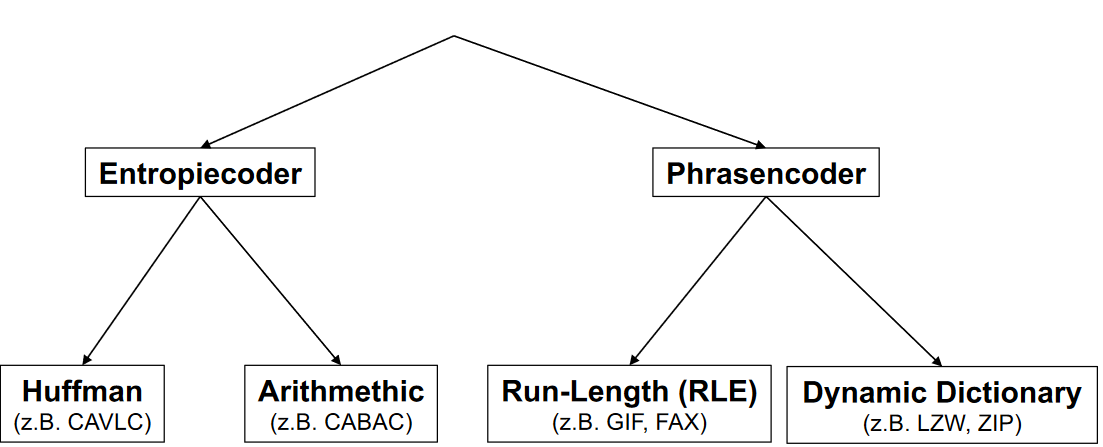
\includegraphics[width=0.75\textwidth]{MMK_RLE.png}
  		  		\caption{Klassifikation von verlustlosen Kompressionsmethoden}
  		  		\cite[Seite 8]{MMK}
  		  		\label{MMK}
  		  	\end{center}
  		  \end{figure}
  		  
  		  
  		  Bei dieser Art der Codierung wird eine Folge von gleichen Zeichen, Buchstaben oder Zahlen durch ein Symbol und die Angabe über die Häufigkeit der gleichen Symbole substituiert. Die Abfolge von identischen Zeichen und der Länge der jeweiligen Sequenz, die in einem sogenannten Run Counter gespeichert wird, wird als \textbf{Run}  und die Anzahl der Wiederholungen werden als Lauflänge beziehungsweise \textbf{Run Length} bezeichnet.
  		  
  		  \begin{equation}
  		  	\text{Aufeinanderfolgende Vorkommen eines Datensatzes} \; d = Run
  		  \end{equation}
  	  
  	      \begin{equation}
  	  	    \text{Anzahl der Wiederholungen} \; n \;\text{von} \; d = RunLength
  	      \end{equation}
  	      \\
  	      Diese Form der Kompression eignet sich unter anderem sehr gut um Redundanzen in Grafiken und Bilddateien mit wenigen Farben zu beseitigen.
  	  
  		  Ist die zu komprimierende Grafik sehr detailreich, besitzt also sehr viele Farben oder Kontraste, ist die Lauflängencodierung nicht mehr geeignet,  da so nur sehr selten gleiche Zeichen in einer Sequenz aufeinander folgen.\cite{ITWissen.info} Auch für Texte eignet sich diese Methode eher nicht, da hier zwar Farben eine untergeordnete Rolle spielen, jedoch die aufeinander folgenden Buchstaben sehr selten gleich sind und so einzelne Zeichen nicht effizient zusammengefasst werden können.\cite[Seite 61]{Lange2021}
  		  
  		  Bei der \textbf{Kompression} werden identische Zeichen so lange eingelesen, bis sich eines ändert - Zeichen und Anzahl die gleich sind, werden festgehalten. Während der \textbf{Dekompression} wird der festgehaltene Wert ausgelesen und die dementsprechende Anzahl an Bits ausgegeben.\cite{ITWissen.info} Der von der Informationsquelle gesandte Datensatz ist verlustfrei wieder hergestellt.
  		  
  		  Sendet die Quelle neben beispielsweise Buchstaben auch Ziffern, muss das Verfahren um Sonderzeichen erweitert werden, so dass die resultierende Angabe weiterhin eindeutig als Lauflänge gekennzeichnet ist. \cite[Seite 62]{Lange2021} Ein Beispiel zur Verdeutlichung findet sich in Abbildung \ref{Lange}.
  		  
  		   \begin{figure} [H]
  		  	\begin{center}
  		  		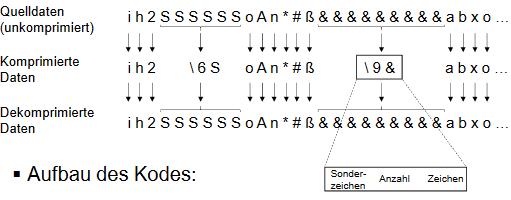
\includegraphics[width=0.75\textwidth]{alpha_ziffer.png}
  		  		\caption{Beispiel Verfahrenserweiterung}
  		  		\cite[Seite 62]{Lange2021}
  		  		\label{Lange}
  		  	\end{center}
  		  \end{figure}
  		  
  		  In der Abbildung \ref{Lange} enthält der Datensatz Buchstaben, Ziffern und  Zeichen. Damit dennoch sinnvolle Sequenzen zusammengefasst werden und der Speicherbedarf verringert werden kann, wird in diesem Beispiel mit dem Sonderzeichen \textit{backslash} codiert.
  		  
  		  Der Kompressionsgrad von Run-Length Encoding hängt stark von der Charakteristik der Quelldaten ab. \cite[Seite 62]{Lange2021} Wie sich dieser äußert wird im folgenden Abschnitt  \textbf{Einsatz \& Anwendungsbeispiele} verdeutlicht.
  	
		\section{Einsatz \& Anwendungsbeispiele}
		Die Lauflängencodierung findet Anwendung bei verschiedenen Grafikdateiformaten, wie beispielsweise dem TIFF\footnote{TIFF = Tagged Image File Format, Standardformat für Druckproduktion}, dem TGA\footnote{Targa Image File, z.B. Vorschaubild}- und dem Bitmap\footnote{Grafik, die von einzelnen Pixeln in einem Raster dargestellt werden}- Dateiformat. In diesem Kapitel werden  Beispiele aus unterschiedlichen Bereichen dargestellt, um zu veranschaulichen, wo sich die Lauflängencodierung eignet und wie sie angewandt wird.
	
		Im Bereich der \textbf{Computergrafik} wird das RLE- Verfahren bei speicherintensiven Rastergrafiken angewendet und ist besonders effizient, wenn es sich um Grafiken mit wenigen aber großflächigen Farben handelt. Hierbei wird die Methode auf die RGB-Farbwerte übertragen. Der Vorgang kann dabei sogar noch verbessert werden, in dem eine Wegoptimierung durch die Wahl des effektivsten Laufweges anhand eines Algorithmus vorgenommen wird.  Dieser Laufweg könnte beispielsweise zeilen-sequenziell, Zick-Zack oder mäanderförmig\footnote{Mäander = Bezeichnung einer Flussschlinge in einer Abfolge weiterer Flussschlingen } (Abbildung \ref{mäander}) sein.
		
		 \begin{figure} [H]
			\begin{center}
				\includegraphics[width=0.25\textwidth]{Mäander.png}
				\caption{Wegoptimierung \textit{mäanderförmig}}
				\cite{kocerheiztech}
				\label{mäander}
			\end{center}
		\end{figure}
	  
		In der Abbildung \ref{Effizienz} werden zwei 48 Byte Grafiken dargestellt und die Effizienz der Datenkomprimierung unter Anwendung von RLE verglichen. Linksseitig befinden sich die Grafiken untereinander und rechts daneben der zugehörige RLE-Code. Die RGB-Farbwerte stellen die zu sehenden Farben dar - sind viele gleichfarbige Pixel (hier als Kästchen dargestellt) aufeinander folgend, können diese gut zusammengefasst werden, in dem die Anzahl vor dem Farbwert übertragen wird. 
			
		In dieser Grafik  wird  schnell deutlich, dass ein detailreicheres Bild ungeeigneter für die RLE-Codierung ist, da kaum gleichfarbige Pixel aufeinander folgen. Die Datenreduktion beträgt im oberen Grafikbeispiel gerade einmal 11\%. In der unteren, in der sich sehr viele nebeneinander liegende blaue Pixel befinden, beträgt die Datenreduktion effiziente 55\%.
				
		\begin{figure} [H]
				\begin{center}
						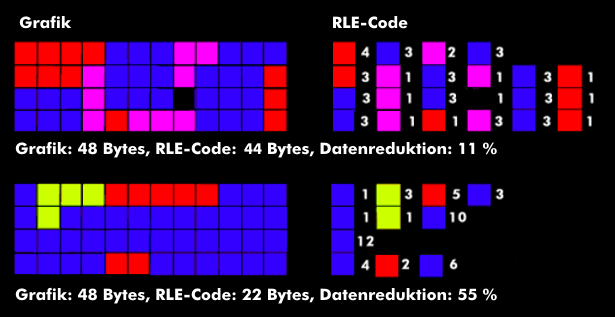
\includegraphics[width=0.75\textwidth]{g_h_Effizienz.png}
						\caption{Beispiel mit geringer und höherer Effizienz}
						\cite{ITWissen.info}
						\label{Effizienz}
					\end{center}
				\end{figure}
		

		Diese Art der Kompression lässt sich nicht nur auf Grafiken anwenden, sondern auch auf Zeichenketten, wie beispielsweise die \textbf{Abfolge bestimmter Nukleinbasen}. Hierbei werden anstatt der RGB-Farbwerte ASCII- Zeichen genutzt.  Im folgenden Beispiel wird die Sequenz der Nukleinbasen (A, C, G , U) zur Verdeutlichung codiert und ausgewertet.\cite{Juchim2021}

		Als Beispieldatensatz dient die Basenabfolge \textbf{A G G U A} C G  .., wobei auf Grund der Übersichtlichkeit nur die ersten 5 Zeichen codiert und ausgewertet werden. Der dazugehörige binäre \textit{ASCII-Code} lautet dementsprechend \textbf{01000001 01000111 01000111 01010101 01000001 } und ist bereits bei nur 5 Buchstaben sehr lang.
		Es wäre nun möglich eine eigene binäre Codierung vorzunehmen, da in diesem Beispiel nur vier unterschiedliche Zeichen (Buchstaben) auftauchen, würden 2 Bit für eine eindeutige Zuordnung ausreichen: 
			
		\begin{table} [H]
				\begin{center}
				\centering
				\begin{tabular}{lllll}
					Position  & Binär & Zeichen &  &  \\
					0 & 00    & A       &  &  \\
					1 & 01    & C       &  &  \\
					2 & 10    & G       &  & \\
					3 & 11	  & U
				\end{tabular}
			\caption{Zuordnungstabelle für Beispiel-Zeichen}
			\end{center}
			\end{table}
	   
	    Dadurch würde sich die betrachtete Sequenz auf \textbf{00 10 10 11 00} kürzen. Die Kompressionsrate ist bereits hier merklich gestiegen, wurden zuvor noch 8 Bit benötigt, sind es jetzt nur noch 2, was bedeutet, dass der erforderlicher Speicherplatz auf 25\% komprimiert werden konnte. Jedoch darf hierbei nicht vergessen werden, dass die Zuordnungstabelle bisher nur dem Sender bekannt ist, diese muss für eine Dekompression allerdings auch dem Empfänger bekannt sein - Daher muss die Tabelle beispielsweise im  Dateikopf mit übertragen werden. Das entspricht daher einen tatsächlichen Bedarf von $4 * (2 +8)$ Bit $= 40$ Bit allein für die Tabelle - bis hier würde sich bei dieser Übertragung wider erwartend eher ein Nachteil ergeben (Bei der Kürze des hier genutzten Datensatzes).
		
		Da die binäre Codierung ineffizient zu sein scheint, wird nun zum Vergleich mit der  \textbf{RLE-Methode} und ebenfalls 2 Bit codiert um einen Vergleich herzustellen: 
		
				\begin{table} [H]
				\begin{center}
					\centering
					\begin{tabular}{ll|llll}
						Code  & Zeichen & Code & Anzahl & &  \\ 
						00 & A    & 00    & 1   &  &  \\
						01 & C    & 01   & 2  &  &  \\
				     	10 & G    & 10    & 3  &  & \\
						11 & U	  & 11   & 4
						
					\end{tabular}
					\label{RLE}		
					\caption{2-Bit RLE-Codiertabelle für Beispiel-Zeichen}
				\end{center}
				\end{table}
		
		Daraus ergibt sich  \textbf{1}A \textbf{2}G  \textbf{1}U \textbf{1}A. Es wird deutlich, dass sich der zu übertragende Datensatz merklich verkürzt hat, in dem die jeweilige Anzahl der aufeinanderfolgenden Buchstaben angegeben wird. Bei der Übertragung wird zuerst die Anzahl und dann das dazugehörige Zeichen gesendet.Der Speicherbedarf reduziert sich hierbei  auf $32$ Bit + Dateikopf. Auf den ersten Blick wüsste man jedoch nicht, ob es sich gerade um eine Zahl oder einen Buchstaben handelt.  \textit{Merke:} Ob beispielsweise eine 01 als C oder als 2 interpretiert wird, wird durch die Position der Zeichenkette festgelegt. 
			
		Es empfiehlt sich die RLE-Methode zu optimieren, um so noch effizientere Ergebnisse zu erzielen. Hierbei werden die Einsen vor den Buchstaben  entfernt, da diese unnötig Speicherkapazität brauchen und zudem keinen Beitrag zur Aussagekraft leisten. Des Weiteren bietet sich die Idee an, eine gemeinsame Codiertabelle mit 3 Bit zu erstellen, um Verwechslungen gänzlich zu vermeiden:
			
				\begin{table} [H]
				\begin{center}
					\centering
					\begin{tabular}{llll}
						Binär  & Zeichen &  &  \\
						000 & A       &  &  \\
						001 & C          &  &  \\
						010 & G          &  & \\
						011 & U	  & & \\
						100 & 2 & & \\
						101 & 3 & & \\
						110 & 4
						
					\end{tabular}
					\label{CT}		
					\caption{3-Bit RLE-Codiertabelle für Beispiel-Zeichen}
				\end{center}
			\end{table}
		
		Daraus resultiert ein komprimierter Datenstrom mit A \textbf{2}G U A . Die Größe des Dateikopfes verringert sich ebenfalls, da die Tabelle, die zum Decodieren mit gesandt werden muss, nun kleiner  ist: $6 * 3$ Bit $= 18 $ Bit $+$ Dateikopf.
		
		Die Beispiele könnten  in unterschiedlichsten Ausmaßen weiter geführt werden, jedoch liegt der Fokus hierbei darauf, ein Verständnis der Funktionsweise in unterschiedlichen Anwendungsgebieten zu vermitteln. Ebenfalls konnten durch die aufgeführten Beispielszenarien bereits erste Vor- und Nachteile angedeutet werden, welche im nächsten Abschnitt zusammengefasst  werden.
	
 		\section{Vor- und Nachteile gegenüber anderen Verfahren}
 		
 		Das RLE-Verfahren zeichnet sich durch seine Geschwindigkeit sowie Einfachheit bei der Implementierung aus und ermöglicht zudem  eine signifikante Datenkompression, wie im vorherigen Kapitel \textbf{Einsatz \& Anwendungsbeispiele} veranschaulicht wird. Zudem gehört sie zu den verlustfreien Kompressionsmethoden, die bei der Dekomprimierung eine vollständige Wiederherstellung des gesendeten Datensatzes ermöglicht.
 		
 		Auch wenn RLE nennenswerte Vorteile bietet, ist es jedoch zur Kompression komplexer\footnote{komplex hier im Sinne von detailreich oder verrauscht} (Farb-)Bilder sowie Texte ungeeignet- auch wenn das Verfahren weiterentwickelt wurde und dadurch die Zunahme des Datenvolumens bei Reihen ohne Wiederholungen kein Problem mehr darstellt, so sind die Kompressionsraten bei solchen Bildern doch denkbar schlecht. \cite{Koeck2006} Der sinnvolle Einsatz von RLE beschränkt sich daher auf Datenströme, die über einen nennenswerten Anteil an \textbf{Runs} verfügt.	Bei sehr kleinen Zeichenfolgen kann es passieren, dass sich die Daten sogar vergrößern. Hierbei müsste vorher eine Mindestanzahl von Werten die zusammengefügt werden sollen, gesetzt werden, um zu ermitteln, ab wann  bei einem vorgesehen Einsatz die Lauflängencodierung sinnvoll ist oder sogar eine Verschlechterung zu erwarten wäre.
		
	
	
	
	\chapter{Fazit}
	An den aufgeführten Anwendungsbeispielen wird deutlich, dass dieses Codierverfahren nicht perfekt ist, jedoch bereits einen ursprünglich hohen Speicherplatzbedarf deutlich komprimieren  und der Datensatz ohne Verluste wieder dekomprimiert werden kann.
	
	Derzeit ist leider noch kein perfektes Codierverfahren bekannt - aber vielleicht kommt dieses noch!
	
	\chapter{Eigenständigkeitserklärung}
	
	Hiermit versichere ich, dass ich die vorliegende Belegarbeit selbstständig und nur unter
	Verwendung der angegebenen Quellen und Hilfsmittel verfasst habe. Die Arbeit wurde bisher
	in gleicher oder ähnlicher Form keiner anderen Prüfungsbehörde vorgelegt.
	
	\vskip 1cm
	
	Berlin, den \date{\today}
	
	\vskip 1.5cm
	\begin{figure} [H]
			
\includegraphics[width=0.5\textwidth]{mgo.png}
	\end{figure}
	Monique Golnik
	
	\addcontentsline{toc}{chapter}{Abbildungsverzeichnis}	
	\listoffigures
	\addcontentsline{toc}{chapter}{Tabellenverzeichnis}	
	\listoftables
%	\printbibliography[heading=bibintoc]
	\printbibliography[heading=bibintoc, title={Quellenverzeichnis}]

	
\end{document}
